\documentclass[../main.tex]{subfiles}
\graphicspath{{\subfix{./figs/}}}


\begin{document}

\section{Prelude}
This thesis is part of a larger effort to elucidate the origins of QGP-like signatures in small systems. To understand this small contribution to the body of knowledge, we first introduce the tools of the trade, then dive into the motivations behind the analysis. This will allow us to fully contextualize our findings which are discussed in the next section.

\section{A Brief Word on Histogramming}

In particle and nuclear physics, histograms form the backbone of much of our analysis. This is because we often seek to determine an underlying probability density from data taken over from a large number of events (ie. collisions). Consider a dataset of $N$ particles, each with some transverse momentum $p_T$. To construct a 1-D histogram, the horizontal axis, representing $p_T$ is split into intervals called bins or buckets. The y-axis denotes the frequency and is constant within a given bin. For a $p_T$ distribution, the frequency of any given bin is such that the integral over the frequency in that bin yields the total number of particles with $p_T$ lying in the bin. For a $p_T$ distribution, it is common to denote the frequency as $dN/dp_T$ since, for a total number of counts $N$:

\begin{equation}
    N = \int \frac{dN}{dp_T} dp_T
\end{equation}

For a $2$-dimensional histogram of $p_T$ and $\eta$, we have:

\begin{equation}
    N = \int \int \frac{dN}{dp_T d\eta} dp_T d\eta
\end{equation}

Similary, for arbitrary kinematic variables $x_1,...,x_N$ we can construct an $N$-dimensional histogram where:

\begin{equation}
    N = \int ... \int \frac{dN}{dx_1...dx_N} dx_1...dx_N  
\end{equation}

Often, we assume the uncertainty in each bin is $\sqrt{n}$, where $n$ is the number of counts in a given bin. This comes from the Poisson distribution. While the absolute error in a bin goes as $\sqrt{n}$, the relative error goes as $\sqrt{n}/n = 1/\sqrt{n}$. Thus, a larger sample gives us better statistics. 

\begin{figure}
    \centering
    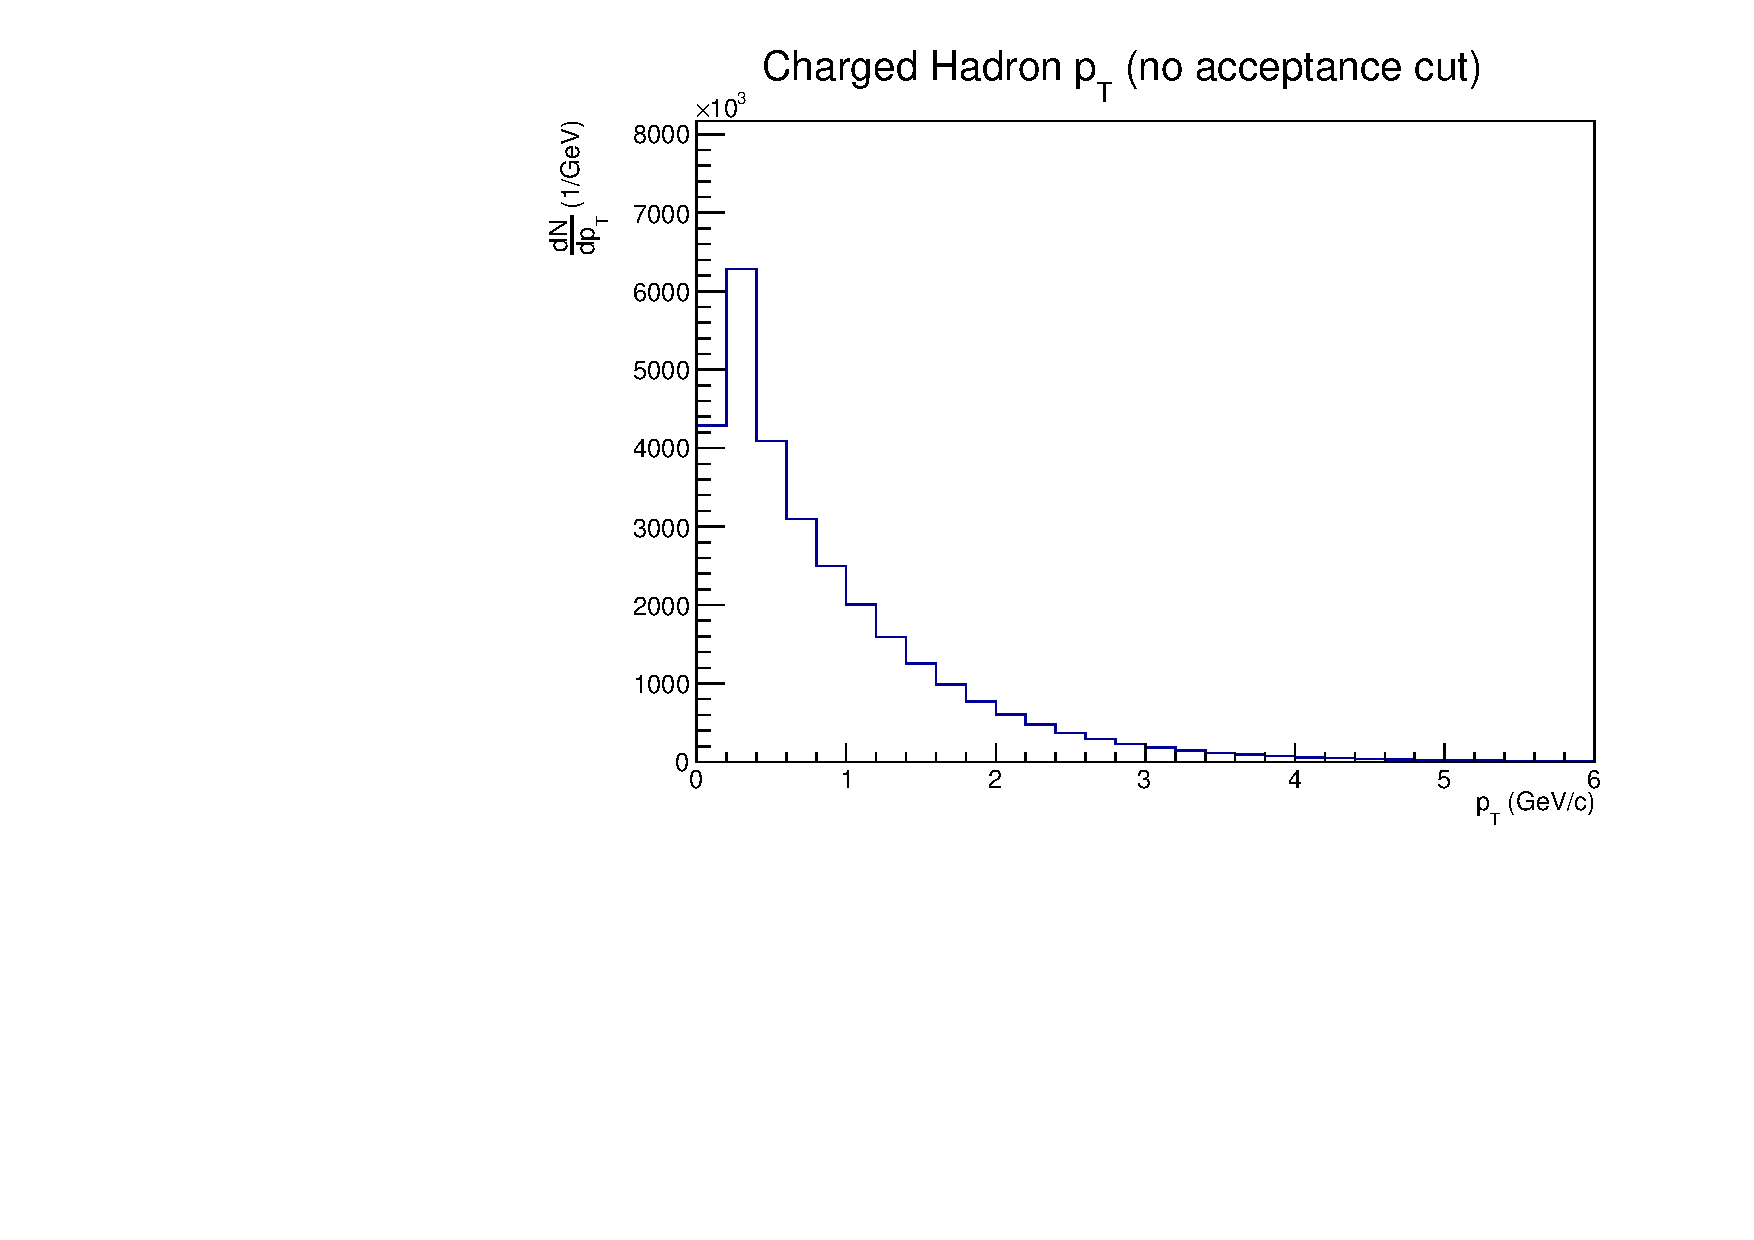
\includegraphics[scale=0.5]{analysis/figs/charged_hadron_pt.pdf}
    \caption{A simple $p_T$ distribution of all charged hadrons from our generated data. Notice how the distribution falls off quickly. This means particles that fall within the momentum range of an associated or a trigger particle are relatively rare.}
    \label{fig:pt_dist}
\end{figure}

\begin{figure}
    \centering
    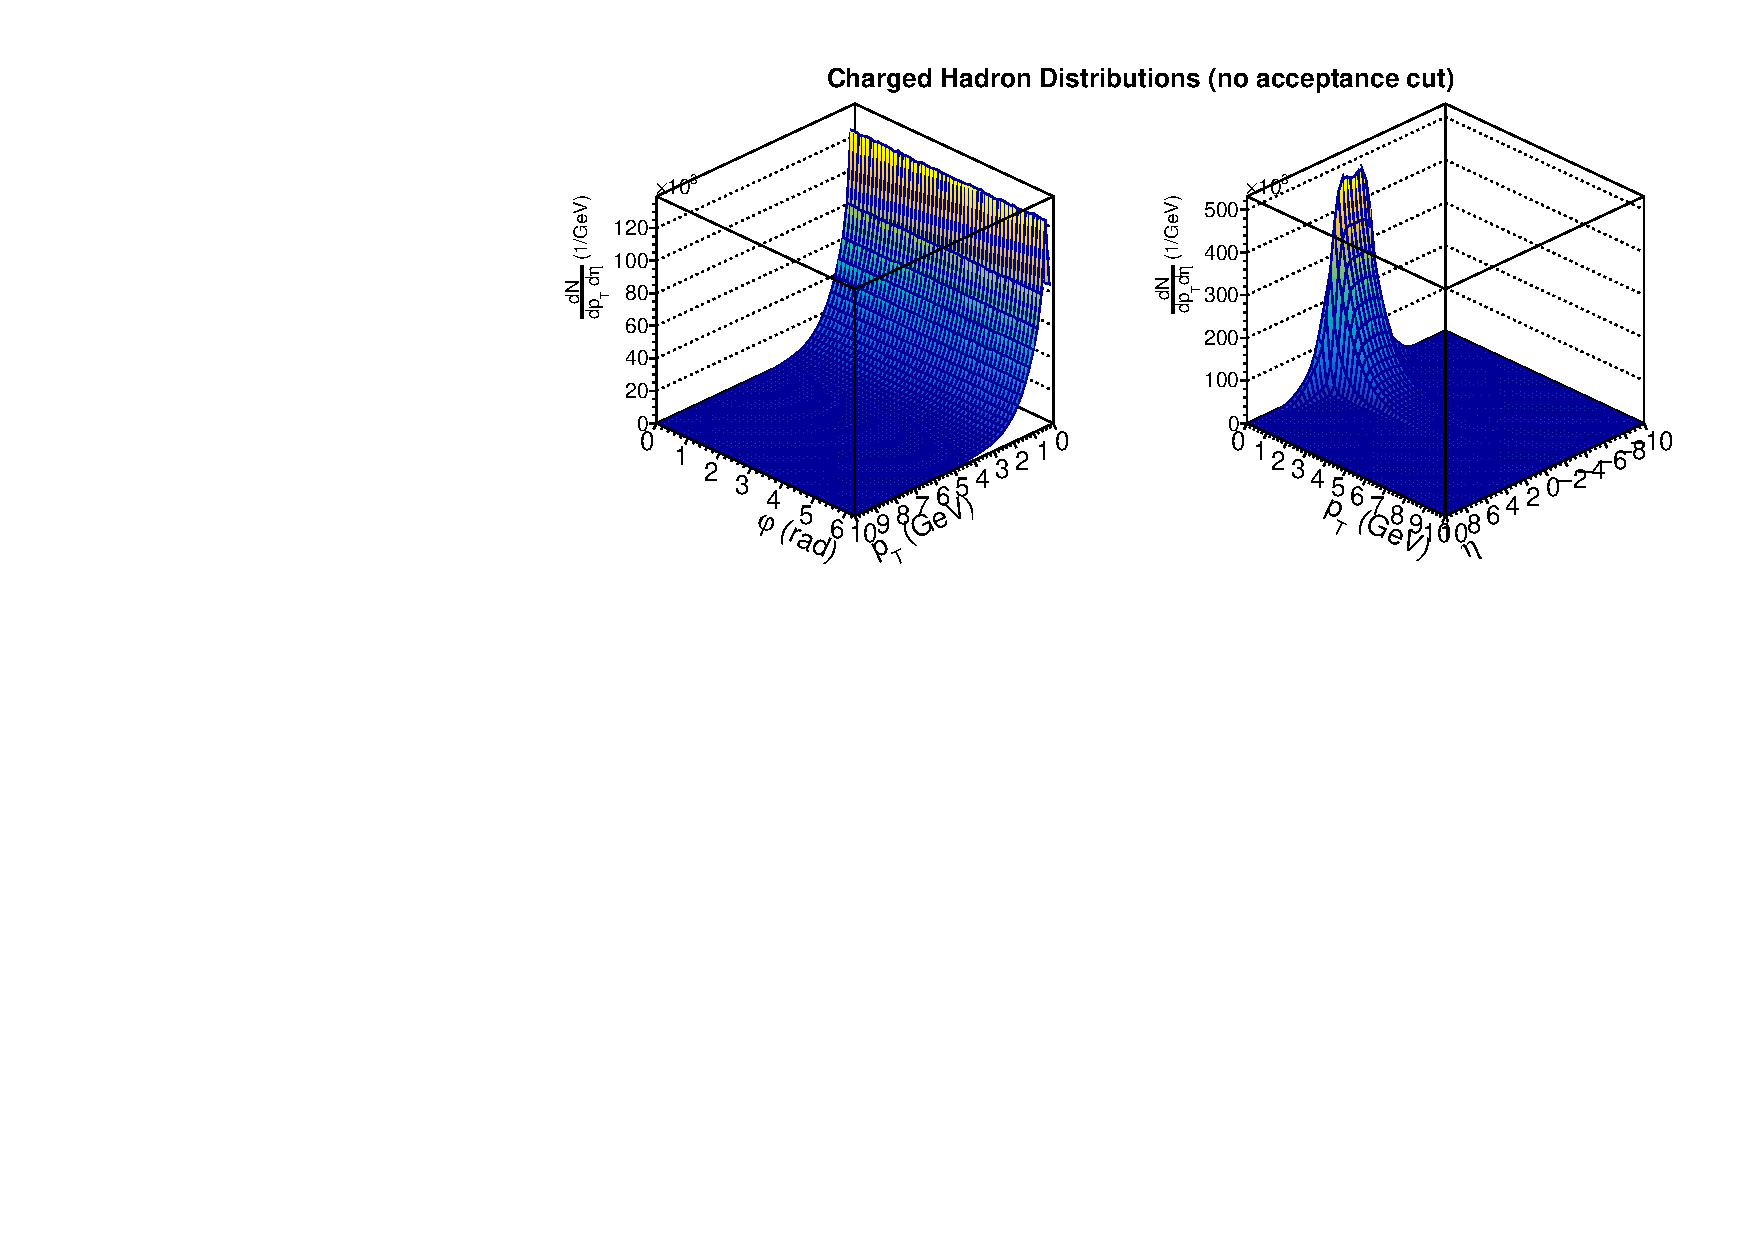
\includegraphics[scale=0.8]{analysis/figs/two_d_dists.pdf}
    \caption{Two two-dimensional histograms. The surface and color represent the counts in a given bin. These distributions are not particularly useful, but they demonstrate how particles are distributed in various kinematic variables. In particular, we see particles are evenly distributed in $\phi$, and particle production is centered at midrapidity.}
    \label{fig:two_d_dist}
\end{figure}

\clearpage
\section{Hadron---$\Lambda$ Angular Correlations}
We are interested in jets because they tell us information about the underlying dynamics between partons. While some physicists fully reconstruct jets to calculate associated observables (eg. two-point energy-energy correlators), we can also gain an understanding of the jet-like structure of events from \textit{two-particle angular correlations}. Rather than performing jet reconstruction, we select for high momentum particles which are assumed to be closely aligned with the jet axis. By correlating these high momentum particles with other particles in the event, we can learn about the structure of jets. To construct an angular correlation, for each event we must:

\begin{enumerate}
    \item Identify high momentum particles within a certain $p_T$ range: $p_T \in [p_T^{\text{trig, min}}, p_T^{\text{trig, max}}]$. These are referred to as the trigger particles and are assumed to be close to the jet axis since they carry a high $p_T$. 
    \item Identify particles within another, typically lower, momentum range $p_T \in [p_T^{\text{assoc, min}}, p_T^{\text{assoc, max}}]$. These are called the associated particles. 
    \item Take the difference in $\varphi$ and $\eta$ for each possible trigger-associated pair. Recall the coordinate system depicted in Fig. \ref{fig:alice_coords}.
    \item Fill a $\Delta\varphi\Delta\eta$ distribution with these angle differences. 
\end{enumerate}


A basic schematic of these steps is shown in Fig. \ref{fig:angular}. Associated particles comoving with the trigger lead to a peak centered on $\Delta\varphi=0$, whereas particles moving in the opposite direction of the trigger lead to a peak centered on $\Delta\varphi=\pi$. These peaks are referred to as the \textit{near-side} and \textit{away-side}, respectively. They are the result of dijets, which are the sprays of hadrons produced from the initial hard scattering. The yields and the widths of these peaks thus tell us about the structure of jets in our events. An event might also contain a background of associated particles that are not correlated with the jet, creating a flat\footnote{In some analyses, flow adds a small sinusoid to the flat background. This is not relevant to our analysis here.} background that the near- and away-side peaks sit on. For example, particles evenly distributed in $\varphi$ would create this background. 

%If the number of associated particles within an event is significantly larger than the number of triggers, this background is largely a combinatorial one, so we call it the \textit{uncorrelated background}. However, if the number of triggers is comparable to the number of associated then we can extract physics from the background, so we call it the \textit{underlying event}. An HFe---hadron (Heavy-Flavor electron) correlation is an example of an angular correlation with an uncorrelated background because producing heavy quarks is difficult due to their mass, so this correlation will have many more associated particles than triggers. In comparison, producing a $\Lambda$ is much easier, so we refer to it as the underlying event in this case. 

\begin{figure}[h]
    \centering
    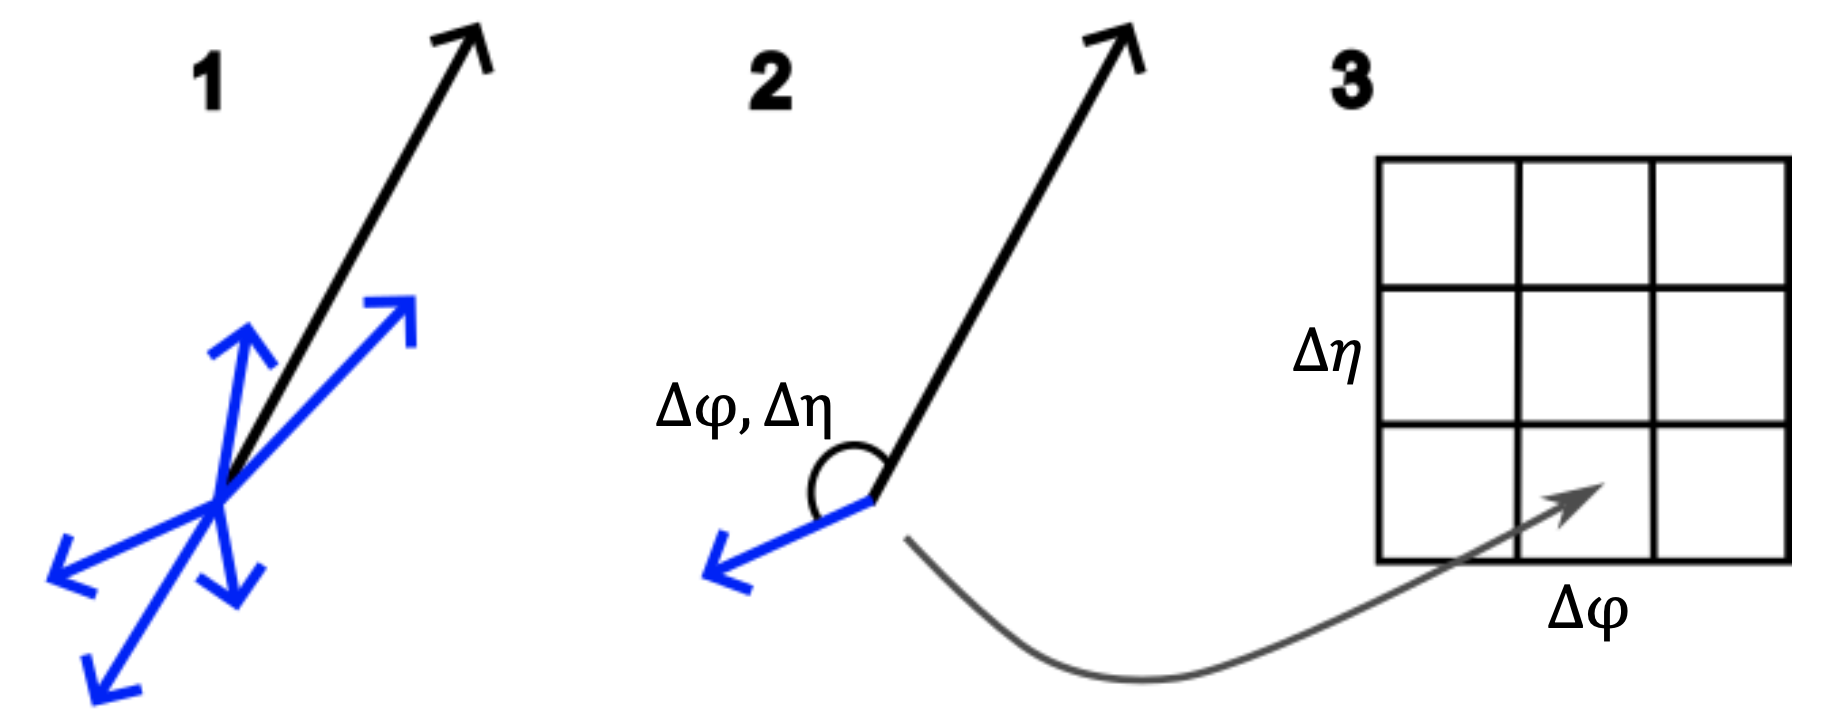
\includegraphics[scale=0.3]{angular_labeled.png}
    \caption{A basic diagram representing how a 2D angular correlation is performed. The black arrow represents a trigger particle and the blue arrows represent associates in the dijet. By taking pairwise differences in $\varphi$ and $\eta$ between the trigger and associated particles, we construct a 2D distribution. Note that typically there is also an uncorrelated background from associated particles that are not in the jet. These are not drawn here for simplicity.}
    \label{fig:angular}
\end{figure}

Broadly, we think of the near- and away-side as representing hard physics from initial interactions involving high four-momentum transfers between partons. The underlying event, which comes from particles not correlated to the jet, originates from two main sources. The first is soft scatterings---additional or secondary scatterings that do not result from the initial hard scattering. For example, a QGP in Pb-Pb would contribute to the underlying event via soft scatterings of partons within the medium. The second source comes from events with multiple hard scatterings or jets. If there are multiple triggers (jets) in the event, then some jet-like signal will contribute to the underlying event. 

\begin{figure}
    \centering
    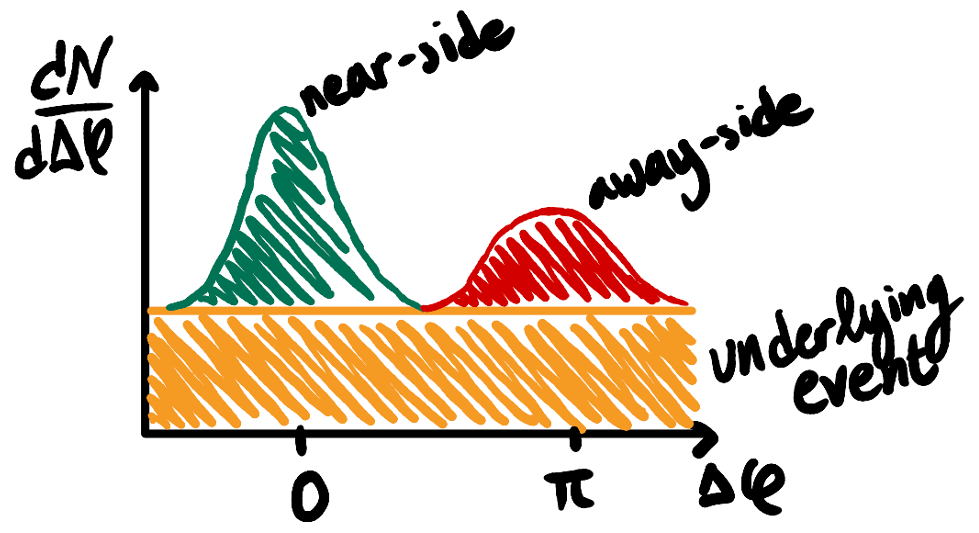
\includegraphics[scale=0.6]{dphi_cartoon.png}
    \caption{A cartoon of an azimuthal correlation. The near-side and away-side represent the jet-like structure of the selected events, and the underlying event gives information about soft physics. }
    \label{fig:dphi_cartoon}
\end{figure}

We select certain particle species to serve as the trigger and associated particles, depending on what physics we are probing. A hadron---hadron correlation utilizes hadrons as the trigger and associated particles while a hadron---$\Lambda$ correlation utilizes hadrons as the trigger and $\Lambda$'s as the associated. Often, we project a $2$D $\Delta\varphi\Delta\eta$ distribution into a $1$D distribution in $\Delta\varphi$. This is referred to as an azimuthal, angular, or $\Delta \varphi$ correlation. For this thesis, we only need the $\Delta\varphi$ distribution; however, structures in $\Delta\eta$ give us important information. 

Typically, the away-side of a $\Delta\varphi$ distribution is wider than the near-side. We can think of dijets as the leading order type of jet that we observe; however, there are also three-pronged pronged jets at next leading order (and so on). Since the trigger defines the jet-axis, the away-side gets smeared by these three-pronged jets. In addition, quarks can radiate gluons and gluons can split, knocking partons off the jet axis and broadening the away-side. 


\begin{figure}
    \centering
    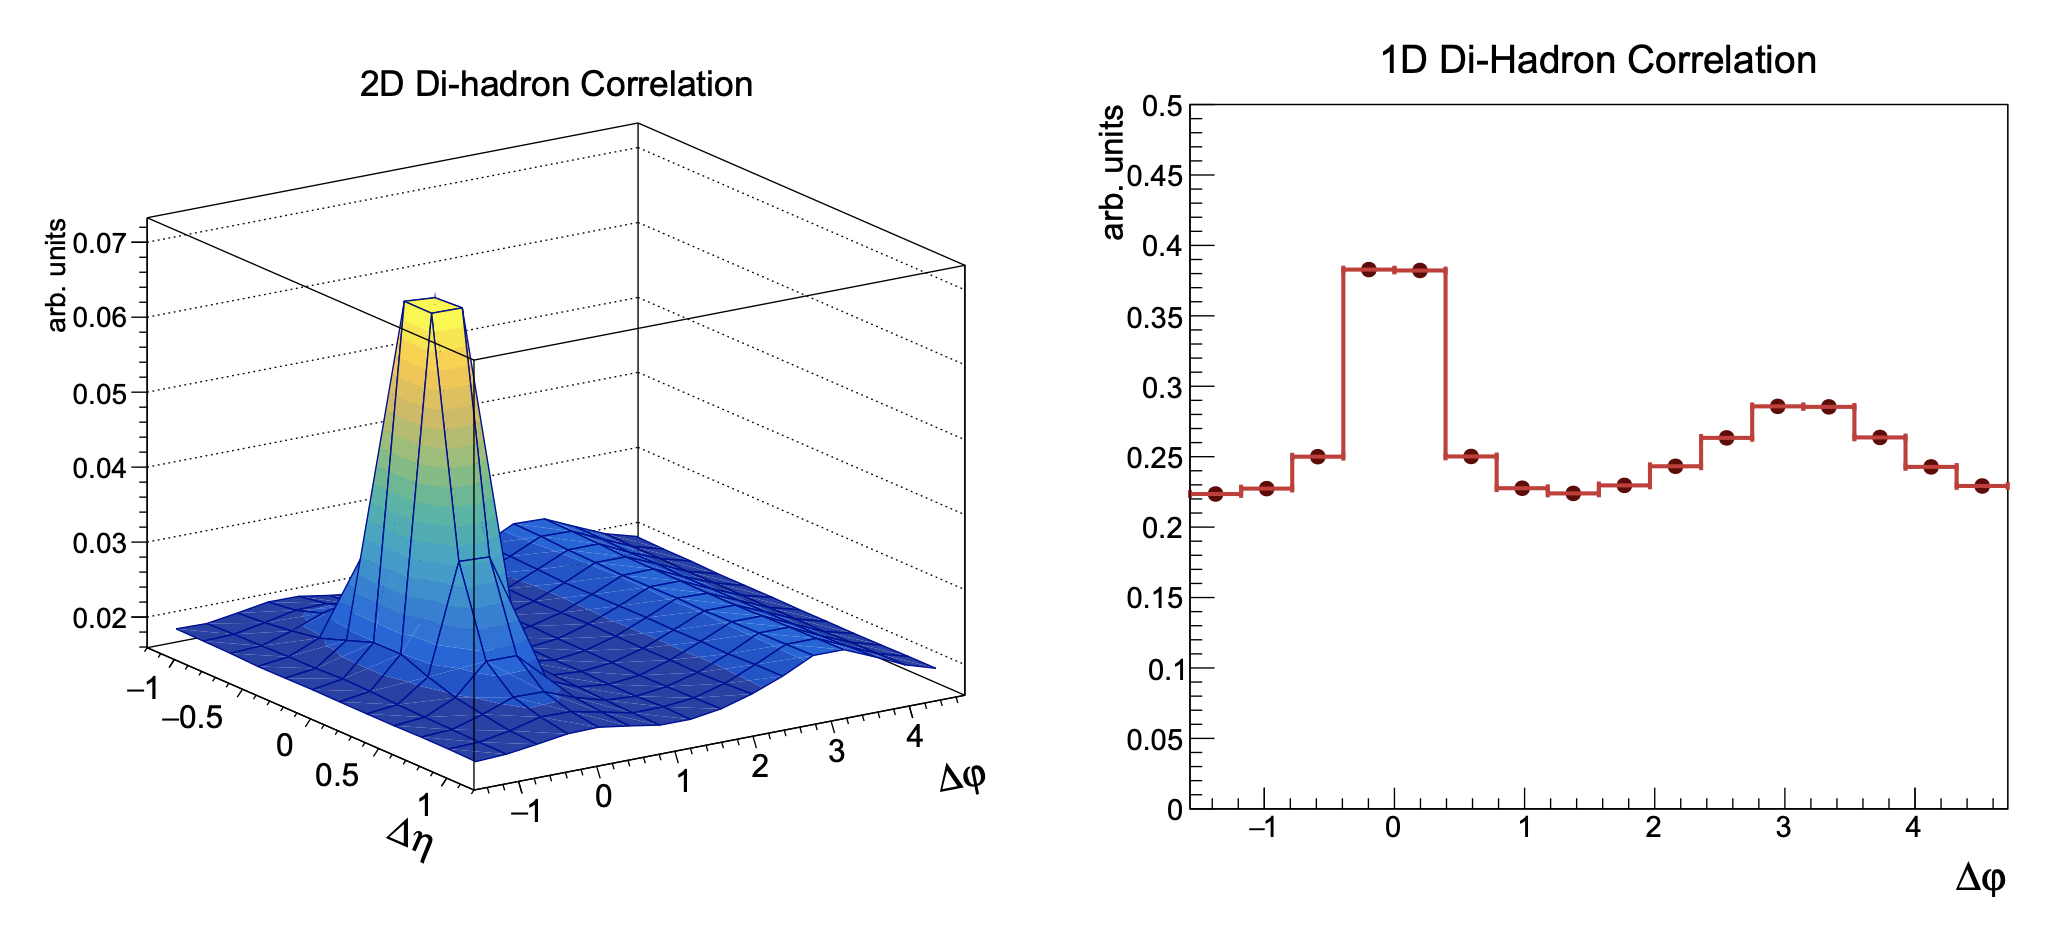
\includegraphics[scale=0.2]{analysis/figs/2dcorr.png}
    \caption{An example of a 2D angular correlation and its projection into a 1D $\Delta\varphi$ distribution. Taken from \cite{Blair:2023rli}.}
    \label{fig:2dcorr}
\end{figure}



\begin{figure}
    \centering
    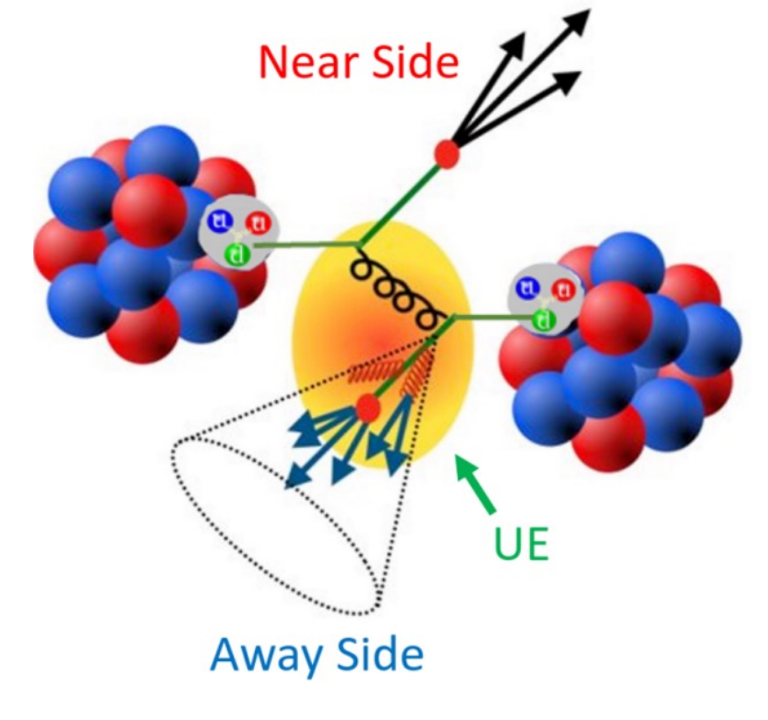
\includegraphics[scale=0.5]{hard_scatter.png}
    \caption{A heavy-ion collision featuring a hard scattering between two partons. This produces two jets, one of which experiences the medium. When we select for events high momentum, we suffer from \textit{surface bias}. This is because dijets that begin near the center of the medium will be fully quenched. It's simply more likely we measure an event where the near-side jet experienced a small path length through the medium while the away-side traveled through a larger length of QGP. This fact is depicted in the cartoon.}
    \label{fig:angular_origins}
\end{figure}

\clearpage
\section{PYTHIA} \label{sxn:pythia}
PYTHIA is an event generator used to simulate high energy collisions. An event is the result of a collision, essentially a list of particles with their kinematic information. To simulate an event, PYTHIA combines both calculations from first principles and ones involving measured parameters---making PYTHIA a data-driven model. In total, PYTHIA relies on the order of $100$ parameters \cite{Bierlich:2022pfr}. Ideally, PYTHIA outputs what an ideal detector would measure, one without a limited acceptance or subject to efficiencies. As a result, PYTHIA is commonly compared with data, allowing high energy physicists to estimate how many particles the detector could not measure and to compare theoretical models with data. 

\begin{figure}[h]
    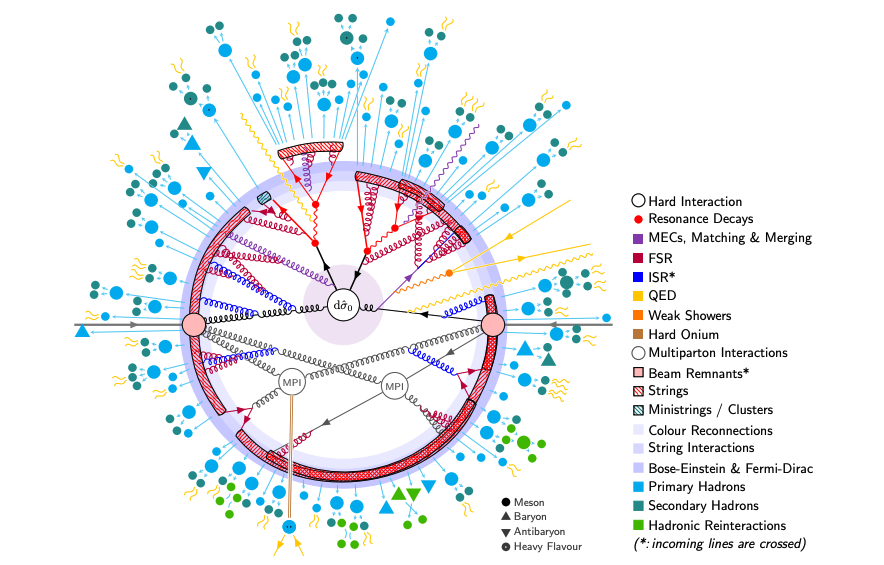
\includegraphics[scale=0.3]{pythia8_event.png}
    \centering
    \caption{The structure of a PYTHIA8 event, decreasing in hardness scale from the initial hard scattering to the final state.}
    \label{fig:pythia}
\end{figure}

%footnote https://www.llnl.gov/article/44656/scientists-now-know-fate-majority-higgs-bosons-particles-produced-lhc#:~:text=Higgs%20bosons%20are%20only%20produced,a%20cascade%20of%20other%20particles.

% http://www.scholarpedia.org/article/Parton_shower_Monte_Carlo_event_generators

% does pythia use FFs and PDFs y

Hadron-hadron collisions are extremely messy, complicated processes, making a full analytic description of such events impossible. Instead, we use numerical methods to generate an event with a certain probability of occuring.\footnote{It's much harder to get a Higgs out of an event, approximately only $1$ in a billion p-p events at the LHC contain a Higgs.} At its heart, PYTHIA relies on Markov Chain Monte Carlo methods which in turn rely on a pseudo-random number generator. In essence, this allows PYTHIA to capture the random nature of events, which are fundamentally subject to quantum mechanical probabilities. There are three "levels" to a given PYTHIA event:

\begin{enumerate}
    \item Process Level: This describes the initial hard-scattering and resonances.\footnote{Short-lived particles like the top quark. These must be produced early in the collision, so they are associated with the initial hard-scattering.} Due to the high $Q^2$, this level relies on pertrubative methods. 
    \item Parton Level: This describes the evolution of the parton shower and multi-parton interactions. This level yields the partonic structure of jets and the underlying event. 
    \item Hadron Level: This handles the confinement of partons into hadrons. Hadronization is modeled by QCD strings that fragment into hadrons. These hadrons can then undergo further decays and scatterings. Hadronization cannot rely on perturbative models. This level yields the hadrons an ideal detector would measure. 
\end{enumerate}

A diagram of a PYTHIA event is shown in Fig. \ref{fig:pythia}, with the stages ordered by hardness scale, but we can think of this as time. The outermost particles, the final-state hadrons, should capture what an ideal detector would measure. PYTHIA is incredibly complex, with multiple layers. Simulating the evolution of partons into color-neutral hadrons is not trivial. 


\section{Motivation}
%trigger selects physics, want hard scatter at midrapidity. vary cut on associate. 

%mixed event doesnt tell you about the physics. have cut in delta eta bc finite acceptance, so lose particles outside that acceptance. if the physics, the pair production, is different in those regions, it affects the widths and shapes of our distributions. thts physics. mixed event wont give you that info, it just gives the prob you lost an associate given you found a trigger. 

This thesis complements an ALICE PhD dissertation that sought to measure strangeness production in and out of jets in p-Pb events at the LHC. This is motivated by the discovery of collective effects in small systems like p-p and p-Pb which questions our understanding of QGP formation and heavy-ion collisions. High multiplicity p-Pb collisions at the LHC show the same strangeness enhancement as low multiplicity Pb-Pb (Fig. \ref{fig: s_enhacement}), prompting us to investigate the origins of strangeness enhancement. By probing the mechanisms behind strangeness production in p-Pb, we can better understand strangeness enhancement, contributing to our understanding of the limits of QGP formation.  

As part of this ALICE study, h-$\Lambda$ correlations were constructed from ALICE p-Pb data. Taking the $\Lambda$ hyperon as the associated allows for calculating the yields of strange particles inside of jets (the near- and away-side peaks) and outside of jets (underlying event). The strangeness production in the underlying event represents soft processes\footnote{Assuming nearly all selected events have one trigger, which was verified.}, which allows us to probe possible QGP formation by separating strangeness enhancement into three distinct regions. In addition, the widths of the near- and away-side were calculated from fits. Since strangeness enhancement is evaluated relative to non-strange hadron production, h-h correlations were also constructed. The ratios of widths and yields---strange over non-strange---were evaluated as a function of multiplicity. This enabled an evaluation of strangeness enhancement. This type of analysis was first performed on the $\phi(1020)$ meson, an $s\bar{s}$ pair \cite{Blair:2023rli}. The $\phi(1020)$ has closed strangeness ($|S|=0$), while the $\Lambda^0$ has $|S|=1$, which makes comparisons between the measurements of both species interesting. 

Due to the finite acceptance of ALICE, this analysis required a cut of $|\eta| < 0.8$. This is smaller than the acceptance of the TPC to avoid edge effects. If strangeness production outside of this acceptance is different from production inside, this would alter our correlations, requiring us to perform corrections. Since hadron collisions are complicated, we do not know \textit{a priori} if this effect is negligible. We have to perform a systematic check with a model like PYTHIA. 

\section{Analysis Description}
In this thesis, we analyze the effect of detector acceptance on h-$\Lambda$ angular correlations. To accomplish this, we first generated $10$ million PYTHIA6 p-p events at $\sqrt{s}=7$ TeV. These events are biased to have virtually no underlying event, meaning that all final-state hadrons result from the hard scattering. This allows for clear separation of the near- and away-side. Out of \textit{all} particles produced in our events, we obtained approximately $15\%$ $\pi^{\pm}$, $11\%$ $\pi^0$, $4\%$ K$^{\pm}$, $4\%$ K$^{0}$, $0.3\%$ protons, and $2\%$ electrons.  

We then construct h---$\Lambda$ and h---h distributions for three acceptances, represented by a pseudorapidity cut on the associate: $|\eta_{\text{assoc}}| < 0.8$, $1.2$, $2.0$. This corresponds to slowly widening the acceptance of the ALICE experiment. The acceptance cut on the trigger is fixed to $|\eta_{\text{trig}}|<0.8$. We fix the cut on the trigger because the trigger selects for the relevant physics, and we are interested in the midrapidity region where particle production from the hard scattering is concentrated. Note that an $\eta$ cut leads to a cut in $\Delta \eta$, but a $\Delta\eta$ cut is not necessarily a cut on $\eta$. We take $4<p_T^{\text{trig}}<8$ GeV/c and $2<p_T^{\text{assoc}}<4$ GeV/c. From Fig. \ref{fig:pt_dist}, we see particles within these $p_T$ ranges are relatively rare. By hadron, we refer to charged hadrons, specifically protons, $\text{K}^{\pm}$, $\pi^{\pm}$, electrons, and their corresponding antiparticles. This is simply because ALICE primarily measures charged particles. By $\Lambda$, we mean the $\Lambda^0$ and its antiparticle. The selection of particle species is consistent with the previously mentioned analysis. For each acceptance, we calculate the ratio of the near- and away-side widths and yields between the h---$\Lambda$ and h---h distributions. We take the ratio because we are interested in the relative production of $\Lambda$ hyperons to hadrons. Recalling the Wroblewski ratio, since the final-state charged hadrons are mostly $\pi^{\pm}$ this is comparable to other measurements of strangeness enhancement. 

\begin{figure}[h]%
    \centering
    \subfloat[\centering Example $\eta$ distribution.]{{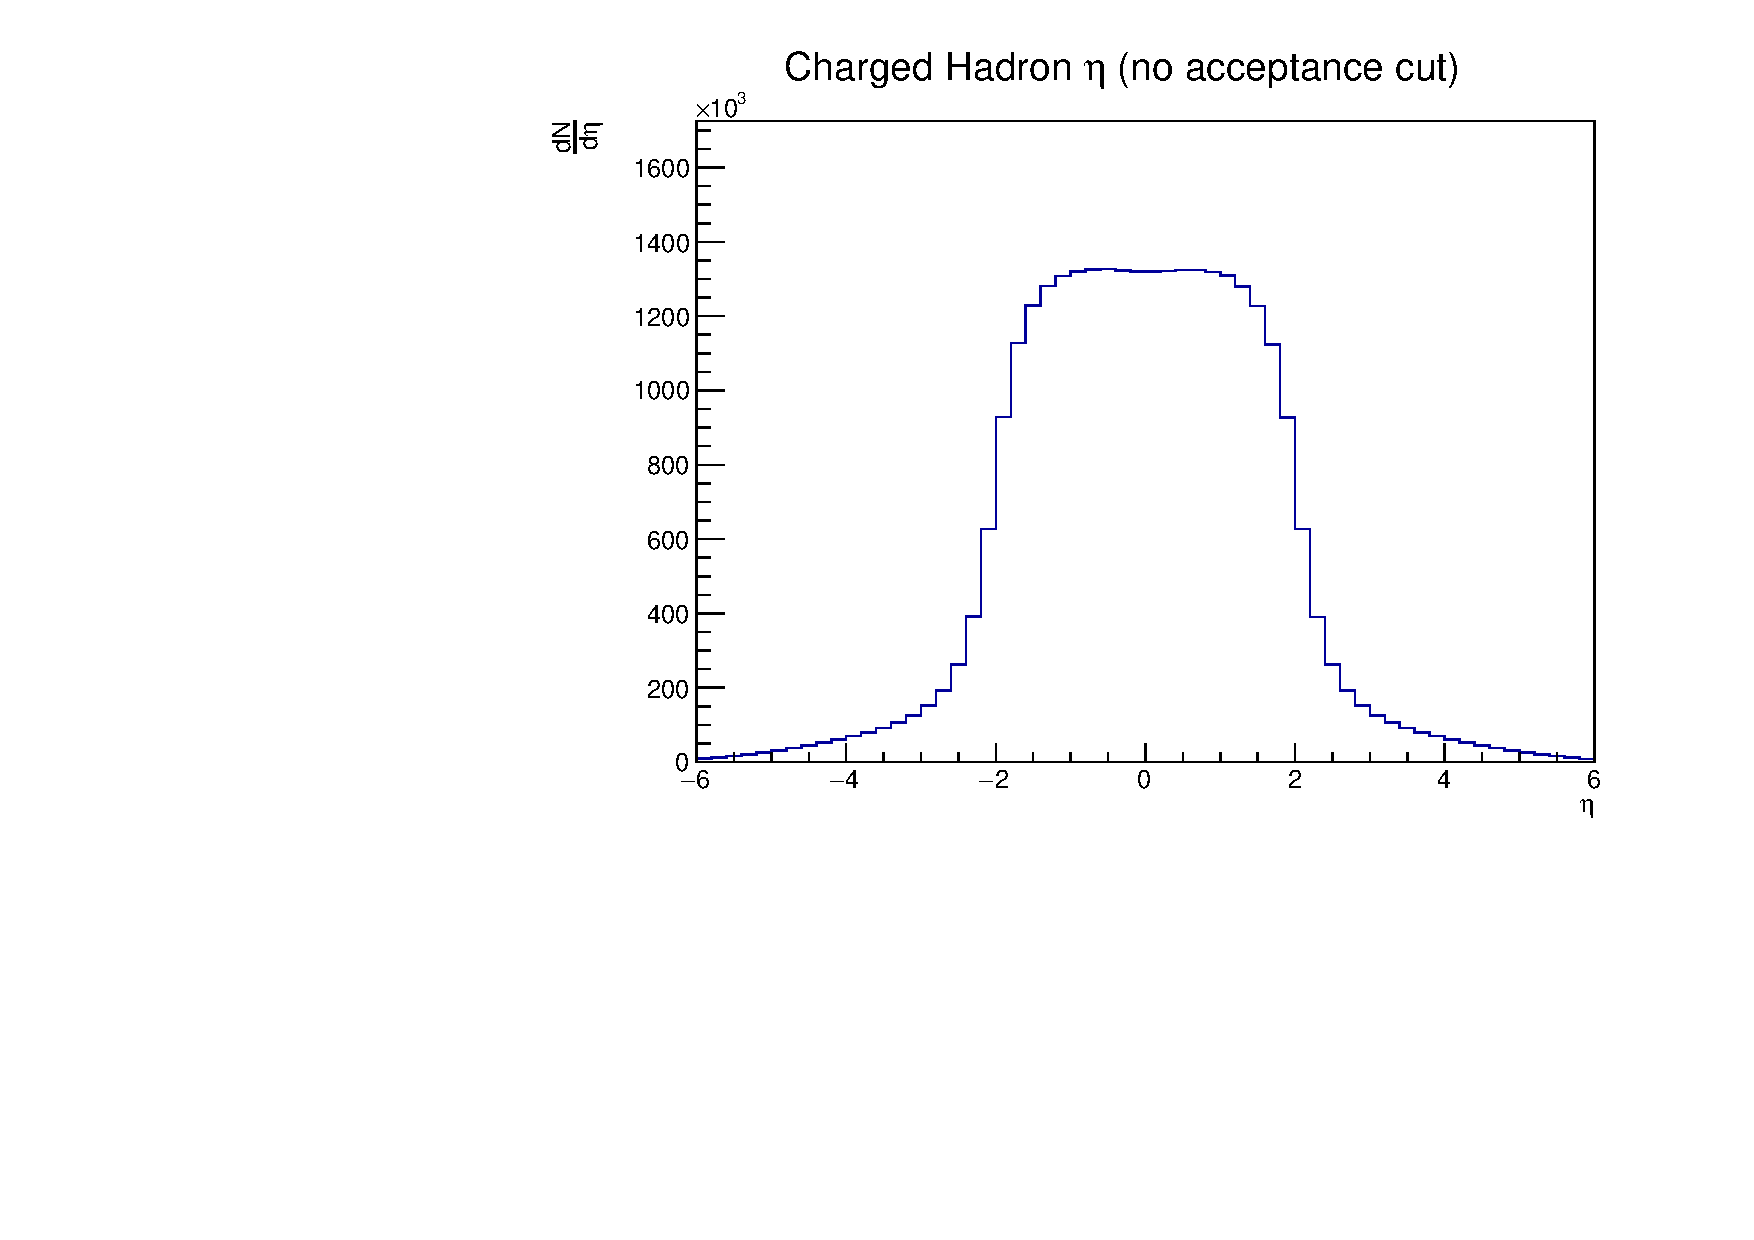
\includegraphics[scale=0.35]{analysis/figs/charged_hadron_eta.pdf} }}%
    \qquad
    \subfloat[\centering Example $\varphi$ distribution.]{{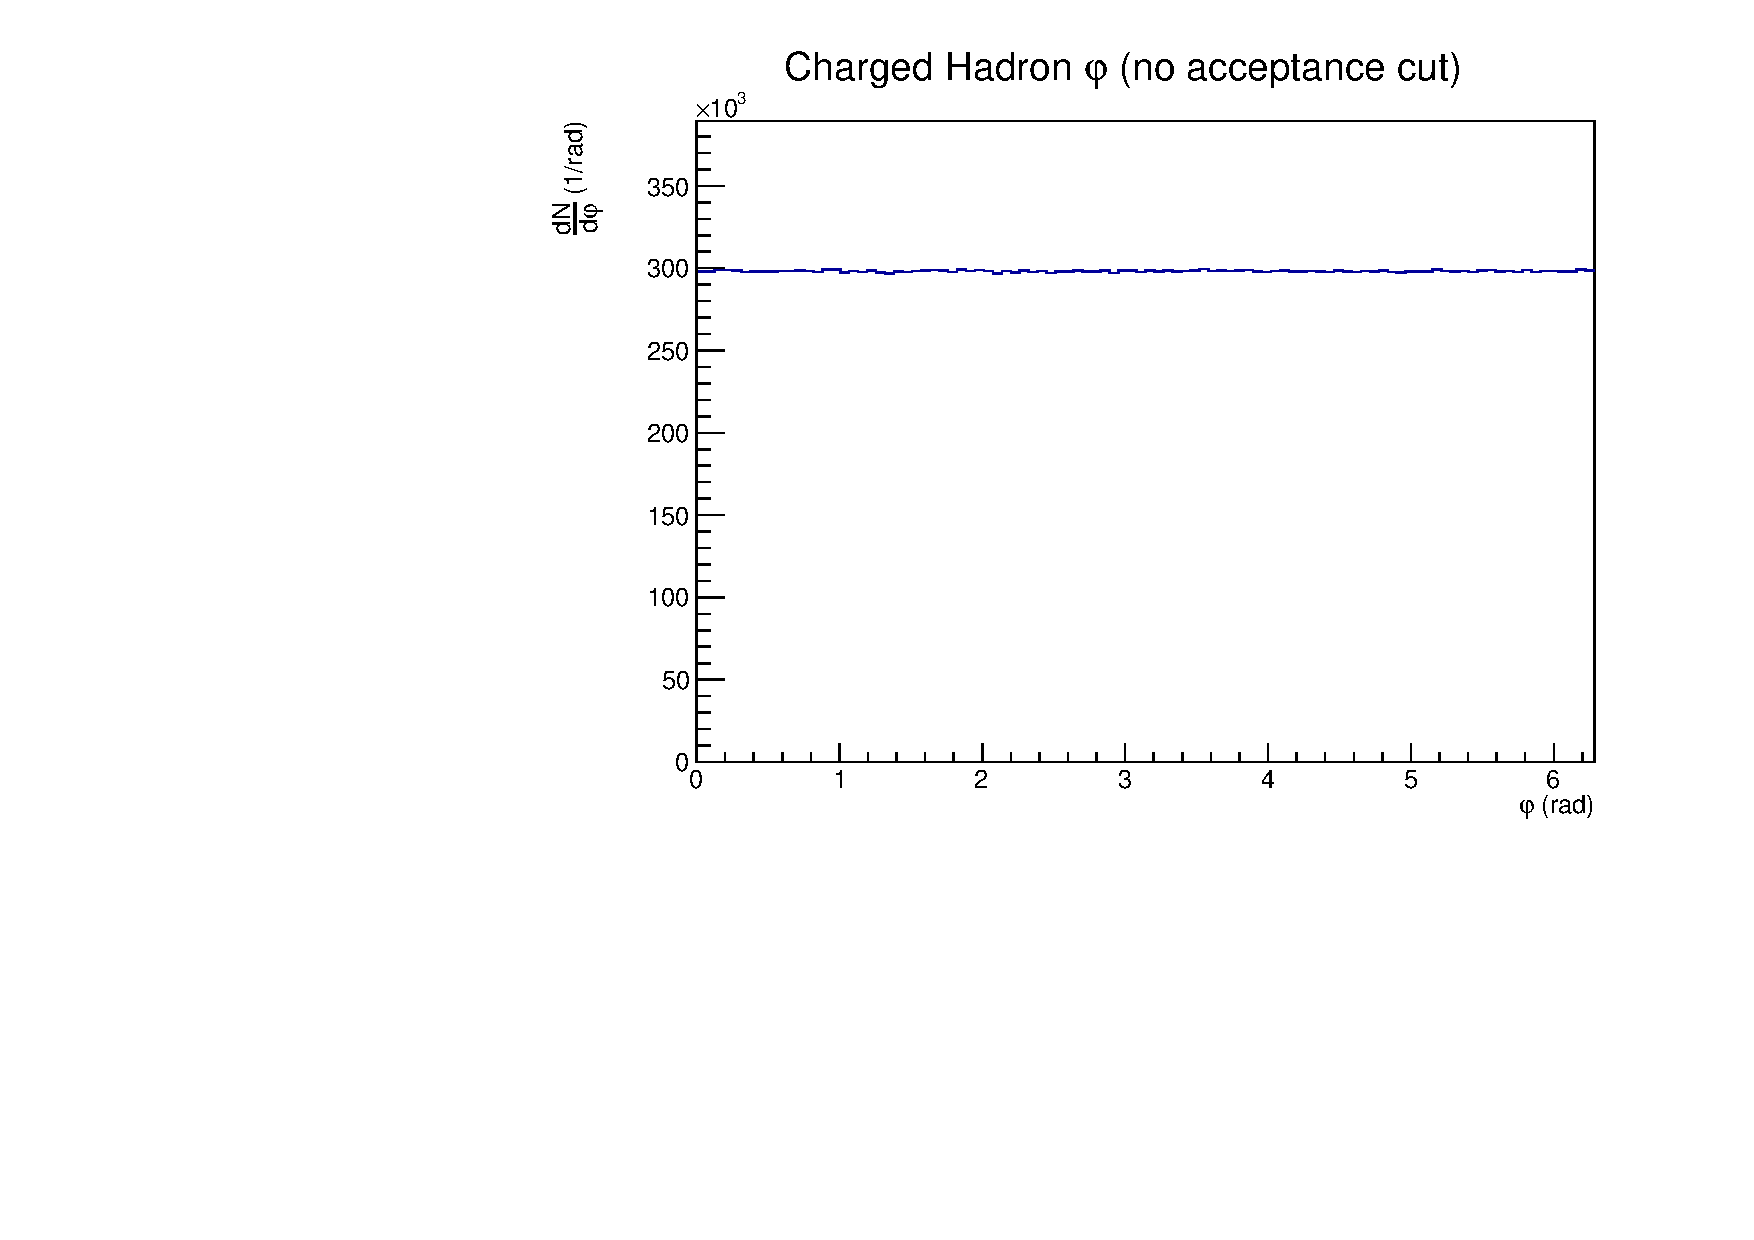
\includegraphics[scale=0.35]{analysis/figs/charged_hadron_phi.pdf} }}%
    \caption{Example distributions of $\eta$ and $\varphi$, constructed with charged hadrons from our generated events. A cut on $\eta$ would chop the $\eta$ distribution. In addition, notice how $\varphi$ is flat, meaning particles are uniformly distributed in the transverse plane.}%
    \label{fig:yield_ratios}%
\end{figure}

Since the selected events have nearly no background, the near- and away-side peaks are clearly separated. Thus, for calculating yields, the near-side is taken as all counts within $\Delta \varphi \in [-\frac{\pi}{2}, \frac{\pi}{2}]$ and the away-side is defined as $\Delta \varphi \in [\frac{\pi}{2}, \frac{3\pi}{2}]$. Thus, the yields are defined as:

\begin{equation}
    Y_{\text{NS}} = \int_{-\frac{\pi}{2}}^{\frac{\pi}{2}} \frac{dN}{d \Delta \varphi} d\Delta\varphi
\end{equation}

\begin{equation}
    Y_{\text{AS}} = \int_{\frac{\pi}{2}}^{\frac{3\pi}{2}} \frac{dN}{d \Delta \varphi} d\Delta\varphi
\end{equation}

where $Y_{\text{NS}}$ is the yield in the near-side peak and $Y_{\text{AS}}$ is the yield in the away-side peak. If the peaks were not so well separated, we would need to define more stringent ranges. Fits are performed with a double Gaussian, and the procedure is outlined below. For each acceptance, we then calculate the ratios: 

\begin{equation}
    \frac{Y^{\text{h}-\Lambda}_\text{NS}}{Y^{\text{h-h}}_\text{NS}} \text{ and } \frac{Y^{\text{h}-\Lambda}_\text{AS}}{Y^{\text{h-h}}_\text{AS}}
\end{equation}

where the superscript represents the type correlation we calculate the yield for. As with the standard measurement of strangeness enhancement, we divide the h---$\Lambda$ distribution by the h---h distribution. Similarly, we assign widths to the near- and away-side peaks via fits. These widths are calculated from the standard deviation of the fit, giving us the ratios:

\begin{equation}
    \frac{\sigma^{\text{h}-\Lambda}_\text{NS}}{\sigma^{\text{h-h}}_\text{NS}} \text{ and } \frac{\sigma^{\text{h}-\Lambda}_\text{AS}}{\sigma^{\text{h-h}}_\text{AS}}
\end{equation}

This fit procedure requires care, so we use the next section to elaborate in detail.

\section{Fitting Procedure} \label{sxn:fits}
While yields can be calculated by simply integrating over each distribution, the widths must be calculated from a fit. To fit each $\Delta\varphi$ distribution, we used the default ROOT fit method which minimizes $\chi^2$:

\begin{equation}
    \chi^2 = \sum_i \left(\frac{y(i) - f(x_i)}{\sigma(i)}\right)
\end{equation}

where $i$ is the bin number, $y(i)$ is the value of the data at bin $i$, $x(i)$ is the bin center, $f$ is the fit function, and $\sigma(i)$ is the error in bin $i$. To characterize the goodness-of-fit, we introduce the idea of the number of degrees of freedom (NDF) for a fit:

\begin{equation}
    \text{NDF} = n - k
\end{equation}

where $n$ is the number of data points and $k$ is the number of free fit parameters. As a rule of thumb, a good fit is one where $\chi^2/\text{NDF} \approx 1$. We display $\chi^2/\text{NDF}$ on all fits. 

To ascribe a width to our distributions, we chose a double Gaussian as our fit function:

\begin{align}
    \frac{dN}{d\Delta\varphi} = &A_{\text{NS}} \exp{\left(\frac{-1}{2}\left(\frac{\Delta\varphi-\mu_{\text{NS}}}{\sigma_{\text{NS}}}\right)^2\right)} \\
    &+ A_{\text{AS}} \exp{\left(\frac{-1}{2}\left(\frac{\Delta\varphi-\mu_{\text{AS}}}{\sigma_{\text{AS}}}\right)^2\right)} 
\end{align}

where $A$ is the amplitude of each Gaussian, $\mu$ is the mean of each Gaussian, and $\sigma$ is the standard deviation of each Gaussian. Since each Gaussian is fitting a peak that originates from the jet-like structure of the events, we fix $\mu_{\text{NS}}=0$ and $\mu_{\text{AS}}=\pi$. This physics consideration reduces the degrees of freedom in the fit by $2$. In Fig. \ref{fig:fit_examples}, we show an example of this fit. The standard deviation of a Gaussian gives us the measure of its width. While a Gaussian fit function is a natural choice, it is not the only one. To ensure the fits are stable and accurately capture the width of the distribution, we also used the generalized Gaussian and Von Mises fit functions. The generalized Gaussian is given by: 

\begin{equation}
    f(x) = \frac{\beta}{2\alpha\Gamma(1/\beta)}\exp{\left(-\left(\frac{|x-\mu|}{\alpha}\right)^\beta\right)}
\end{equation}

where $\beta$ is the shape parameter, $\alpha$ is the scale parameter, $\mu$ gives the location of the mean, and $\Gamma$ is the gamma function. Notice that for $\beta=2$, the generalized Gaussian is the Gaussian distribution. Again, we fit a sum of generalized Gaussians to each $\Delta\varphi$ distribution. As with the double Gaussian, one mean is fixed to $0$ and the other to $\pi$. The standard deviation for the generalized Gaussian is: 

\begin{equation}
    \sigma = \sqrt{\frac{\alpha^2 \Gamma(3/\beta)}{\Gamma(1/\beta)}}
    \label{eq:gengaussigma}
\end{equation}

\begin{figure}
    \centering
    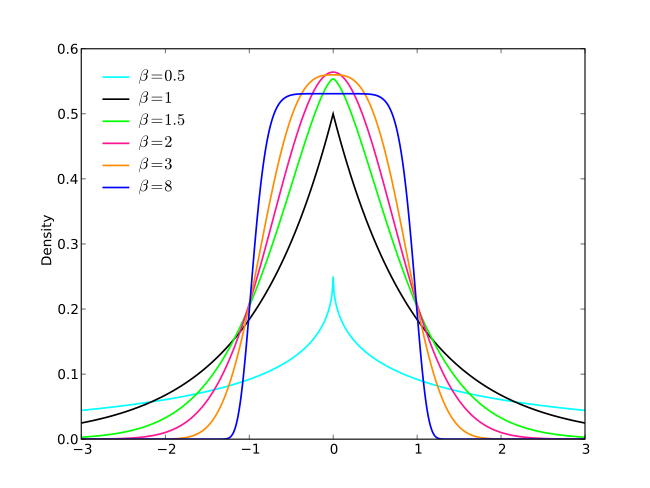
\includegraphics[scale=0.5]{analysis/figs/gengaus.png}
    \caption{A depiction of the generalized gaussian probability density for various values of $\beta$. We see that $
    beta$ controls how sharply peaked the distribution is. From: \textit{Wikipedia}.}
    \label{fig:gengaus}
\end{figure}

Fundamentally, a $\Delta\varphi$ correlation is a distribution wrapped on a circle, which is the focus of \textit{directional statistics}.\footnote{Statistics on the circle is tricky.   Naively, the average of 364$^{\circ}$ and 1$^{\circ}$ is 182.5$^{\circ}$, but we know it should be 0$^{\circ}$.} This is because $\varphi$ is an angle on a circle, so $\Delta \varphi$ is also periodic. Figures like Fig. \ref{fig:dphi_cartoon} are slightly deceptive because they do not explicitly show the distribution is wrapped on the circle. There is no difference between $\Delta \varphi = -\frac{\pi}{2}$ and $\Delta \varphi = \frac{3\pi}{2}$. The Von Mises is a natural choice because it is a periodic approximation to the Gaussian distribution. The Von Mises probability density function is given by

\begin{equation}
    f(x) = \frac{\exp{(\kappa \cos{(x-\mu)})}}{2\pi I_0(\kappa)}
\end{equation}

where $\kappa$ is the concentration parameter, $\mu$ is the location, and $I_0$ is the modified Bessel function of the first kind of order zero. Since $\cos{(x)}$ and $I_0(x)$ are $2\pi$-periodic, the Von Mises distribution is intrinsically periodic, unlike the Gaussian and generalized Gaussian. This makes the Von Mises an appealing choice. From Fig. \ref{fig:vonmises}, we see that $1/\kappa$ is like the standard deviation and $\mu$ is an angle that behaves like the mean. Furthermore, a small value of $\kappa$ corresponds to a uniform distribution (not concentrated), while a large value of $\kappa$ creates a sharply peaked distribution (concentrated). Again, we fix $\mu=0$ for the near-side and $\mu=\pi$ for the away-side. In order to compare widths with the Gaussian and generalized Gaussian fits, we need to translate $\kappa$ into a circular standard deviation. Since we are in the territory of directional statistics, this requires great care. 

\begin{figure}
    \centering
    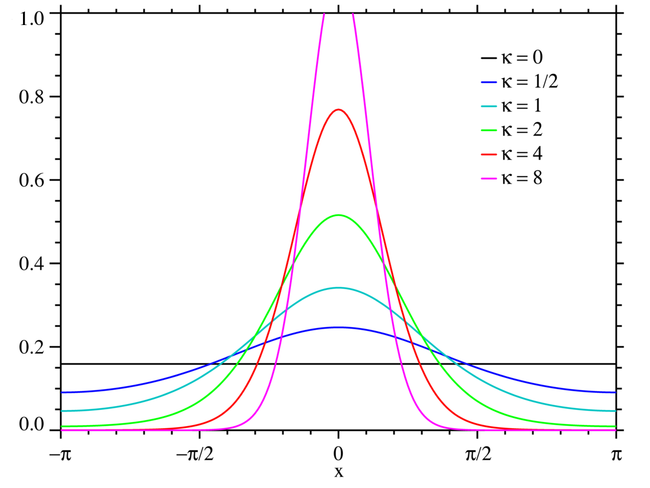
\includegraphics[scale=0.4]{analysis/figs/vonmises.png}
    \caption{The Von Mises distribution for various values of $\kappa$, the concentration parameter. Source: \textit{Wikipedia}.}
    \label{fig:vonmises}
\end{figure}

Consider a finite distribution of points on the unit circle, much like our $\Delta\varphi$ distributions. To characterize the spread of these points, we can associate the position of each point with a vector, and take the sum of these vectors, as shown in Fig. \ref{fig:resultant}. If our points on the circle are highly concentrated, the resultant vector will attain a large magnitude; however, if our points are highly spread, the resultant vector will have a magnitude nearly zero. To quantify this, we define the mean resultant length: 

\begin{equation}
    R = \frac{1}{N} \left|\left|\sum_i \Vec{R}_i \right|\right|
\end{equation}

\begin{figure}
    \centering
    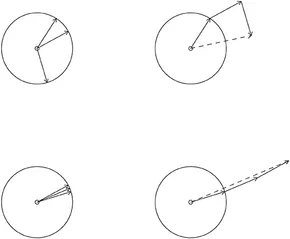
\includegraphics[scale=0.6]{analysis/figs/resultant.png}
    \caption{The left column represents two circular, or directed, datasets. A unit vector points to data points on the circle. By taking the resultant of these unit vectors, we can estimate the spread of the data. Image from \cite{cremers_one_2018}.}
    \label{fig:resultant}
\end{figure}

where $\vec{R_i}$ are the unit vectors representing each data point, and $N$ is the total number of points. This is simply the magnitude of the resultant vector divided by the number of points. One can show that $R \in [0, 1]$, where a value of $R=0$ indicates highly spread data, while a value of $R=1$ corresponds to a highly concentrated dataset. This allows us to define the mean circular variance: 

\begin{equation}
    V = 1-R
\end{equation}

so $V=0$ means concentrated data and $V=1$ represents a spread dataset. This is closer to a typical variance we would associate to a dataset on $\mathbb{R}$. It is important to note that\footnote{However, for $\sigma \ll 1$, $\sigma \approx \sqrt{2V}$. This is obtained from a simple Taylor expansion.}

\begin{equation}
    \sigma \neq \sqrt{V}
\end{equation}

We can extend these ideas to a continuous distribution. For a wrapped normal distribution, a Gaussian in a variable $x \pmod{2\pi}$, we find 

\begin{equation}
    R = \exp{\frac{-1}{2}\sigma^2}
\end{equation}

where $\sigma$ is the circular standard deviation associated with the wrapped normal distribution. Thus, 

\begin{equation}
    \sigma = \sqrt{\ln{(-2 R)}}
    \label{eq:vonmiseswidth}
\end{equation}

The wrapped normal distribution closely approximates the Von Mises distribution, meaning we can use this definition to associate a linear standard deviation to the Von Mises. For the Von Mises distribution, 

\begin{equation}
    R = \frac{I_1(\kappa)}{I_0(\kappa)} \coloneq A_1(\kappa)
\end{equation}

Finally, for the Von Mises, this implies the correct standard deviation is 

\begin{equation}
    \sigma = \sqrt{\ln{(-2 A_1(\kappa)})}
\end{equation}


This is the standard deviation we compute to compare with the Gaussian and generalized Gaussian fits. For all fits, the near- and away-side are simultaneously fitted and the means are fixed. In summary, the standard deviations we use to compare widths between fits are:

\begin{center}
    \bgroup
    \def\arraystretch{1.5}
    \begin{tabular}{|c|c|} \hline
        Fit Function & Standard Deviation \\ 
        \hline
        Gaussian & $\sigma$ \\ 
        Generalized Gaussian & $\sqrt{\frac{\alpha^2 \Gamma(3/\beta)}{\Gamma(1/\beta)}}$ \\
        Von Mises & $\sqrt{\ln{(-2 A_1(\kappa)})}$ \\ 
        \hline
    \end{tabular}
    \egroup
\end{center}

For each acceptance, we calculate the ratios: 

\begin{equation}
    \frac{\sigma^{\text{h}-\Lambda}_\text{NS}}{\sigma^{\text{h-h}}_\text{NS}} \text{ and } \frac{\sigma^{\text{h}-\Lambda}_\text{AS}}{\sigma^{\text{h-h}}_\text{AS}}
\end{equation}

\FloatBarrier
The final results for these ratios are calculated from the double Gaussian fits. In the next section, we also compare these results with the double generalized Gaussian and double Von Mises fits. An example of these fit functions is displayed in Fig. \ref{fig:fit_examples}, which demonstrates the different shapes of each function. For details concering error propagation and all fits, see Appendix \ref{appendix:a}.

\begin{figure}
    \centering
    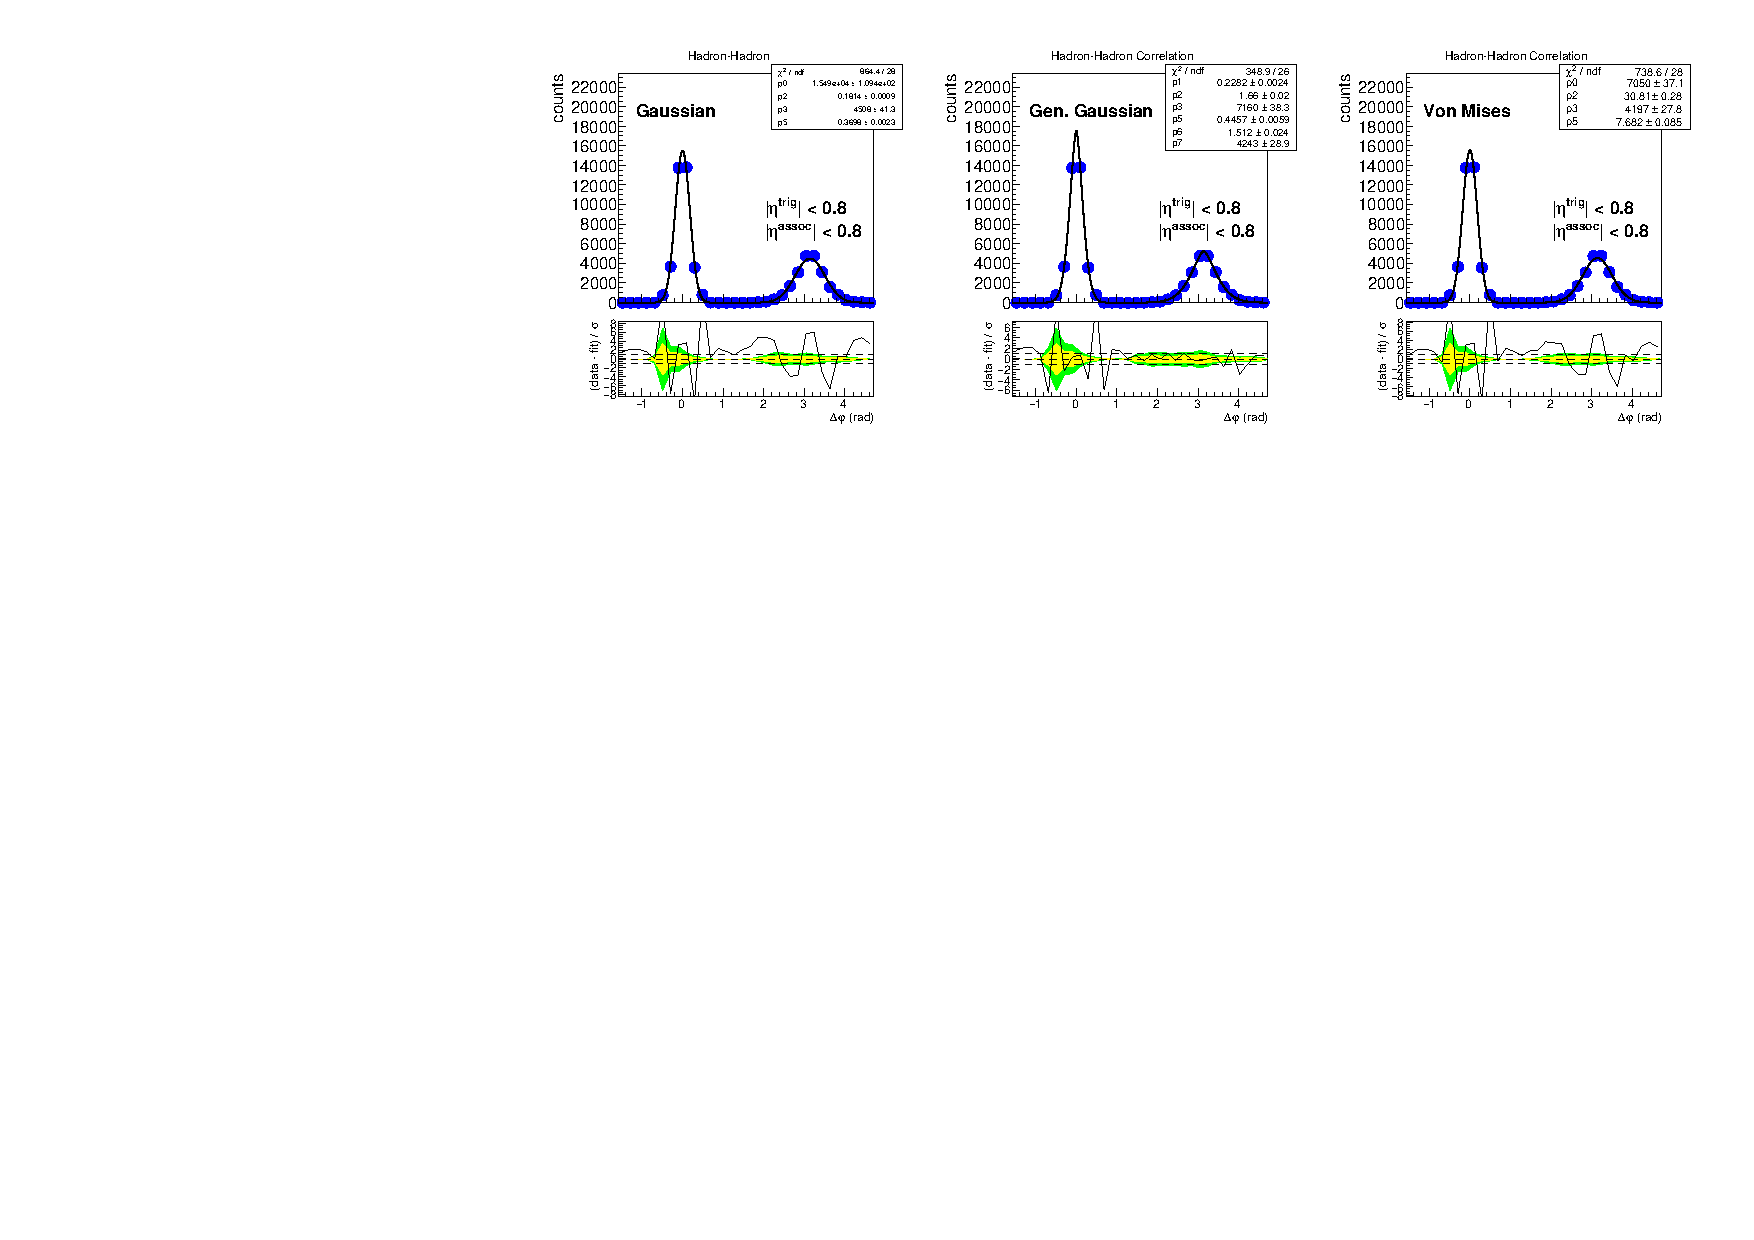
\includegraphics[scale=0.85]{results/figs/example_fits.pdf}
    \caption{Examples of various fits on a h---h distribution with an acceptance cut of $|\eta|<0.8$. The graphs under each distribution represent terms in the $\chi^2$ formula, indicating where the fit describes the data well. The yellow band represents one $\sigma$ and the green band shows two $\sigma$. For this particular correlation, we see the generalized Gaussian describes the away-side quite well. The Gaussian and Von Mises cannot adequately capture the peak of the away-side. Since $\beta \neq 2$, this could indicate the near- and away-side are not truly Gaussian.}
    \label{fig:fit_examples}
\end{figure}
\FloatBarrier

\ifSubfilesClassLoaded{%
    \printbibliography
}

\end{document}